\section{Codon IMM}

A protein can be modelled by a HMM whose states emit amino acids. For example,
Fig.~\ref{fig:core-model} shows a possible HMM architecture for aligning sequences of amino-acids,
for which indels are modelled by insert ($\state{I}$) and delete ($\state{D}$) states and matched
positions are modelled by match ($\state{M}$) states. Each match state defines a potentially
distinct probability distribution over amino acids so as to model position-specific amino acid
frequencies. Insert states might instead define the same background probability distribution over
amino acids. Delete states are silent states and therefore do not emit any amino acid: it represents
position-specific missing amino acids. $\state{B}$ and $\state{E}$ are special states that represent
end start and end of alignment. In particular, the probability of $\state{B}$ being the first state
is one: $p(Q_1=\state{B})=1$.

\begin{figure}[htbp]
  \centering
  \captionsetup{width=.5\linewidth}
  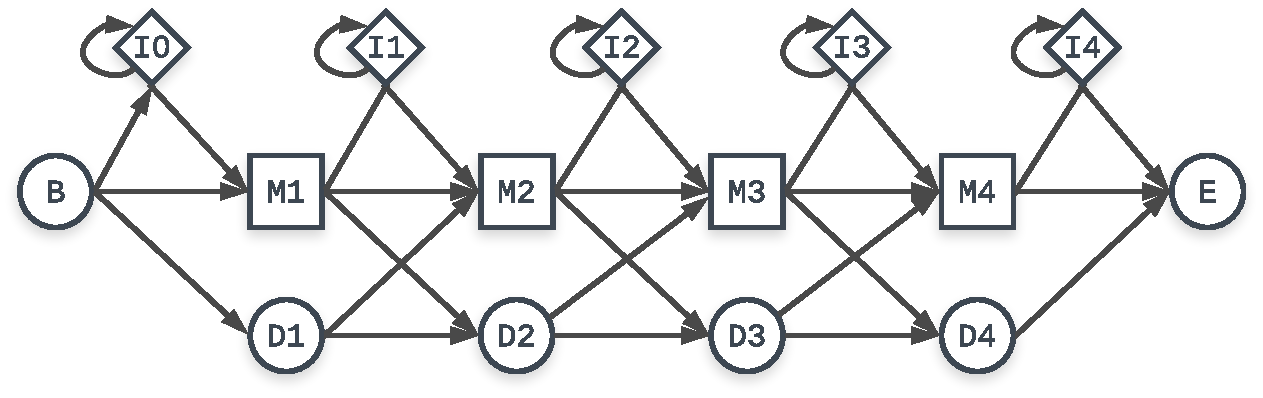
\includegraphics[width=.5\linewidth]{figure/core-model}
  \caption{$\state{B}$ and $\state{E}$ are silent states that denote the start and the end of an
  aligment. States $\state{M}$ represent matches while states $\state{I}$ and $\state{D}$ model
  indels.}\label{fig:core-model}
\end{figure}

HMMs are widely used to model proteins and are used to search for homologous subsequences in target
sequences made of amino acids. However, the researcher ocasionally do not have a ready-to-use amido
acid sequence but instead a sequence of nucleotides that might contain homologous subsequences that
code for proteins. Some residues of those homologous subsquences might be missing or might have been
inserted by whatever reason. Still, one should be able to uncover error-prone subsequences when
compared against to their homologous protein HMMs.

Let $(Q_t, S_t)$ be a HMM with the amino acid alphabet $\set{A}$. We want to replace it by an IMM
that preserves the model architecture (i.e., same set of states, state transitions and initial state
probabilities) but instead have states that emit sequences of nucleotides instead of amino acids
symbols. In particular, the new match and insert states will emit nucleotide sequences that varies
in length from a single nucleotide to five nucleotides. The emission distribution of silent states
(e.g., delete states) will stay the same: probability one of emitting an empty sequence in the IMM
parlance.

Let $\set{B}$ be a nucleotides alphabet (e.g., $\set{B} \eqdef \{\res{A}, \res{C}, \res{G},
\res{T}\}$), and let $\state{M}$ be a state that in the protein HMM would emit an amino acid. From
its amino acid distribution and any other relevant source of information (codon usage bias, for
instance), one can define the probability $p(X_t=x_1x_2x_3 \gv Q_t=\state{M})$ of $\state{M}$
emitting the codon $(x_1, x_2, x_3) \in \set{B}^3$.

\begin{example}
  Suppose that a state $\state{M}$ has the amino acid distribution defined by
  \begin{equation*}
    p(S_t=\res{Y} \gv Q_t=\state{M}) = 0.8 ~~\text{and}~~ p(S_t=\res{C} \gv Q_t=\state{M}) = 0.2,
  \end{equation*}
  where $\res{Y}$ and $\res{C}$ are Tyrosine and Cysteine.
  Based on the canonical genetic code alone, we could define codon distribution as follows:
  \begin{equation*}
    \begin{split}
      p(X_t=\res{TAT}\gv Q_t=\state{M})= 0.8/2, &\quad p(S_t=\res{TAC}\gv Q_t=\state{M})=0.8/2\\
      p(X_t=\res{TGT}\gv Q_t=\state{M})= 0.2/2, &\quad p(S_t=\res{TGC}\gv Q_t=\state{M})=0.2/2,
    \end{split}
  \end{equation*}
  where $\res{A}$, $\res{C}$, $\res{T}$, and $\res{G}$ are nucleotides.
\end{example}

Defining $p(X_t=x_1x_2x_3 \gv Q_t=q_t)$ for every state $q_t \in \set{Q}$ produces an IMM $(Q_t,
X_t)$ that emits codon sequences and, therefore, could in principle be used to evaluate sequences of
nucleotides. However, such model would fail to match sequences that present indels at the base
level: a match state that mainly emits Tyrosine (codons $\res{TAT}$ and $\res{TAC}$ in the canonical
genetic code) should be able to consider the sequence $\res{TAAT}$ as a possible Tyrosine codon that
happens to have a base insertion. We therefore propose an additional modification: the emitted codon
has to go through two steps of (possible) base deletions and two steps of (possible) base insertions. In
each of those steps, there is a probability $\epsilon$ of a modification happening.
\Cref{fig:hmm-to-imm} summarizes the proposed modifications.

\begin{figure}[htbp]
  \centering
  \captionsetup{width=.6\linewidth}
  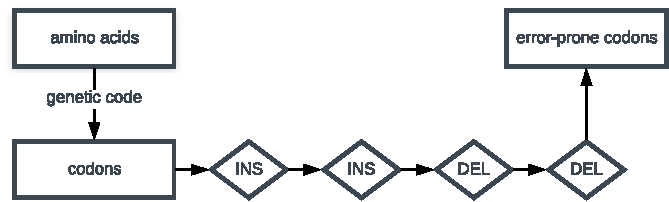
\includegraphics[width=.6\linewidth]{figure/hmm-to-imm}
  \caption{Conversion of protein HMM into codon IMM.\@ Amino acid distributions are first converted
  into codon distributions. Generated codons go through four indels steps, each of which has a
  probability $\epsilon$ of actually happening. At the end, we have a distribution of error-prone
  codons: variable-length sequences having from one to five nucleotides.}\label{fig:hmm-to-imm}
\end{figure}

We will replace the codon emission process by one
that instead produces base sequences of different lengths to account for errors and frame-shifting.

Node $\state{M}_j$ in Fig.~\ref{fig:codon-hmm-tree} represents the modified match state.
The generated codon will go through four transitions, each one representing one of three possibilities: (i) delete a base; (ii) insert a base; or (iii) do nothing.
The deletion can happen in any of the three codon positions with equal probability.
If a deletion has already happened, the next deletion can happen in any of the remaining two positions with equal probability.
The insertion can happen between any two bases, before the first base or after the last base with equal probability.

The codon emitted at node $\state{M}_j$ can go under $m\in\{0, 1, 2, 3, 4\}$ base indels during
the state transitions that end at some leaf-node state.
The probability of it undergoing $m$ indels is given by
\begin{equation*}
  p(M=m) = \binom{4}{4-m} (1 - \eps)^{4-m} \eps^m,
\end{equation*}
where coefficient $\binom{4}{m}$ counts the number of paths corresponding to $m$ base indels.
Fig.~\ref{fig:indel-dist} shows the base indel distributions over different values of $\eps$.
Let $F$ be a random variable representing the final sequence length generated by the model in
Fig.~\ref{fig:codon-hmm-tree}.
We have the probabilities
\begin{equation*}
  \begin{split}
    p(F=1) = p(F=5) &= \eps^2(1-\eps)^2, \\
    p(F=2) = p(F=4) &= 2\eps^3(1-\eps) + 2\eps(1-\eps)^3,~\text{and} \\
    p(F=3)          &= \eps^4 + 4\eps^2(1-\eps)^2 + (1-\eps)^4
  \end{split}
\end{equation*}
illustrated in Fig.~\ref{fig:len-dist} over different values of $\eps$.

\begin{figure}[htbp]
\centering
\begin{subfigure}{.5\textwidth}
  \centering
  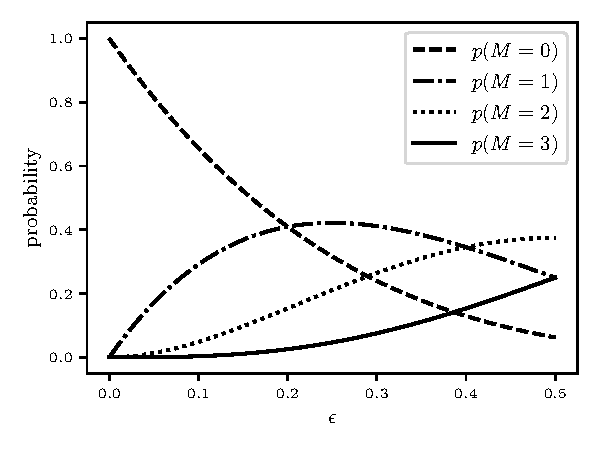
\includegraphics[width=.7\linewidth]{figure/indel-prob}
  \caption{Base indel distribution.}%
  \label{fig:indel-dist}
\end{subfigure}%
\begin{subfigure}{.5\textwidth}
  \centering
  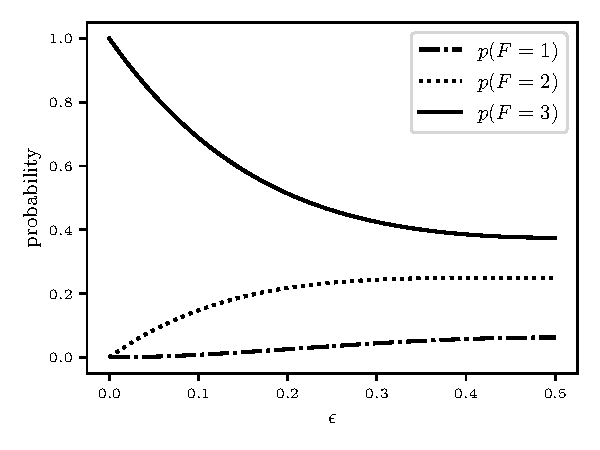
\includegraphics[width=.7\linewidth]{figure/seq-len-prob}
  \caption{Sequence length distribution.}%
  \label{fig:len-dist}
\end{subfigure}
\caption{
    Distribution of base indels and sequence length over the transition probability $\eps$.
    It is recommended to choose a value for $\eps$ that is smaller than $1/5$ such that
    $p(M=m)<p(M=m+1)$, as per Fig.~\ref{fig:indel-dist}.
}\label{fig:dist}
\end{figure}

A sequence $\mathbf z=z_1 z_2\dots$ of finite but variable length will emerge at the end of the
process represented in Fig.~\ref{fig:codon-hmm-tree}.
Let $\mathcal Q_f$ be the set of hidden paths, starting with $Q_t=\state{M}_j$ and ending at some leaf-node state,
that generate sequences of length $f$.
Let $Z^f=(Z^f_1, \dots, Z^f_f)$ be a $f$-tuple of random variables that generates such sequences of length $f$.
We have
\begin{equation*}
  p(Z^f=z_1\dots z_f,F=f) = \sum_{\mathbf q \in \mathcal Q_f}
  \cprob{Z^f=z_1\dots z_f}{Q_{t..t+4}=\mathbf q} p(Q_{t..t+4}=\mathbf q).
\end{equation*}
